% Created 2019-10-23 Wed 12:07
% Intended LaTeX compiler: pdflatex
\documentclass[11pt]{article}
\usepackage[utf8]{inputenc}
\usepackage[T1]{fontenc}
\usepackage{graphicx}
\usepackage{grffile}
\usepackage{longtable}
\usepackage{wrapfig}
\usepackage{rotating}
\usepackage[normalem]{ulem}
\usepackage{amsmath}
\usepackage{textcomp}
\usepackage{amssymb}
\usepackage{capt-of}
\usepackage{hyperref}
\usepackage[margin=0.5in]{geometry}
\usepackage{amsthm}
\usepackage[norsk]{babel}
\theoremstyle{definition}
\newtheorem{definition}{Definisjon}
\newtheorem{task}{Oppgave}
\date{}
\title{Innleveringsoppgaver uke 43}
\hypersetup{
 pdfauthor={Tarjei Bærland},
 pdftitle={Innleveringsoppgaver uke 43},
 pdfkeywords={},
 pdfsubject={},
 pdfcreator={Emacs 26.1 (Org mode 9.1.13)}, 
 pdflang={Norsk}}
\begin{document}

\maketitle
\section*{Et enkelt, dobbelt plot}
\label{sec:orgbd96d91}

Velg to funksjoner og plot de innenfor de samme x-verdiene.

Lever fila som \texttt{f"uke43\_\{fornavn\}\_dobbelplot.py} og den resulterende grafen som \texttt{f"uke43\_\{fornavn\}\_dobbelplot.png}.

\section*{Starten på utforsking av framoverdifferansen}
\label{sec:org36251a4}
Velg én av funksjonene fra forrige oppgave, denne skal du nå gjøre følgende med:

\begin{enumerate}
\item Finn funksjonens deriverte \emph{analytisk}, og opprett denne som en egen funksjon
\item Lag et plot som sammenligner den analytiske løsningen med den numeriske tilnærmingen du finner ved å bruke \emph{framoverdifferanse}-metoden fra sist uke.
\end{enumerate}

\section*{Et eksempel på plotting}
\label{sec:orga002abc}
Om du har tre lister med verdier som skal plottes, en med x-verdier og to med y-verdier, kan du bruke en fremgangsmåte à la følgende for å få til dette.

Inntil videre kan du bruke den følgende fremgangsmåten ukritisk. Bruk hjelpesystemet aktivt om du ønsker å finne andre ting du kan endre med plottene dine, tilstreb ikke å google problemer du eventuelt støter på.


\begin{verbatim}
import matplotlib.pyplot as plt

def f(x):
    return x ** 2 - 5

def g(x):
    return x ** 3 + 13


# Vi lager oss en liste [-10, -9, ..., 0, ... 9, 10]
x_verdier = list(range(-10, 11))

# Vi oppretter tomme lister som skal holde y-verdiene våre
y_verdier1 = []
y_verdier2 = []

# Vi legger funksjonsverdiene til y-verdilistene
for x in x_verdier:
    y_verdier1.append(f(x))
    y_verdier2.append(g(x))

# Vi oppretter et tomt plot
fig, ax = plt.subplots()

# Vi lager oss to linjer, en for hver liste av y-verdier. Legg merke til kommaet
linje1, = ax.plot(x_verdier, y_verdier1)
linje2, = ax.plot(x_verdier, y_verdier2)

ax.set_xlabel('x-verdier')
ax.set_ylabel('y-verdier')
ax.set_xlim(-14, 14)
ax.set_ylim(-500, 600)

# Vi setter navn på linjene våre
ax.legend([linje1, linje2], ['f(x)', 'g(x)'])

fig.savefig('eksempelplot.png')
fig.show()
\end{verbatim}

Som produserer følgende plot: 

\begin{figure}[htbp]
\centering
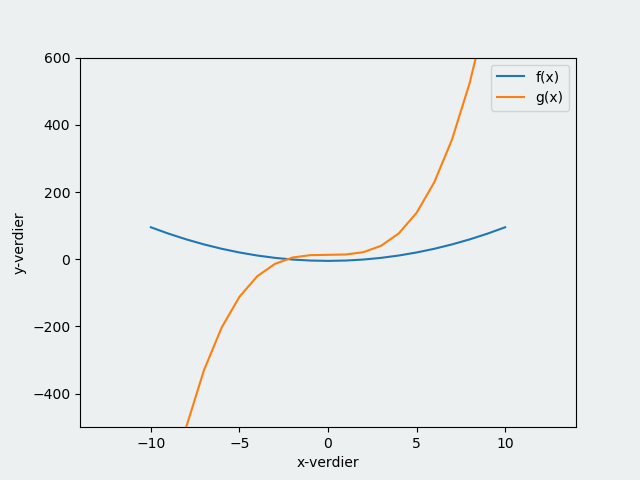
\includegraphics[width=.9\linewidth]{../figurer/uke42_eksempelplot.png}
\caption{Et enkelt, dobbelt plot}
\end{figure}
\end{document}
